%!TEX TS-program = xelatex
%!TEX encoding = UTF-8 Unicode

\documentclass[12pt]{extarticle}
% extarticle is like article but can handle 8pt, 9pt, 10pt, 11pt, 12pt, 14pt, 17pt, and 20pt text

\def \ititle {Descartes}

\def \isubtitle {Lecture 01}

\def \iauthor {Stephen A. Butterfill}
\def \iemail{s.butterfill @warwick.ac.uk}
\date{}

%for strikethrough
\usepackage[normalem]{ulem}

\input{$HOME/latex_imports/preamble_steve_handout}

%\bibpunct{}{}{,}{s}{}{,}  %use superscript TICS style bib
%remove hanging indent for TICS style bib
%TODO doesnt work
\setlength{\bibhang}{0em}
%\setlength{\bibsep}{0.5em}


%itemize bullet should be dash
\renewcommand{\labelitemi}{$-$}

\begin{document}

\begin{multicols*}{3}

\setlength\footnotesep{1em}


\bibliographystyle{newapa} %apalike

%\maketitle
%\tableofcontents




%---------------
%--- start paste
%---------------


      
\def \ititle {Lecture 01}
 
\def \isubtitle {Descartes}
 
\begin{center}
 
{\Large
 
\textbf{\ititle}: \isubtitle
 
}
 
 
 
\iemail %
 
\end{center}
 
\emph{Overall Topic}:
What, according to Descartes, is the relation between a sensory perception and the thing perceived?
 
\emph{Question for this Lecture}: 
How can we acquire knowledge about the essential nature
of the bodies located outside us?
 
\emph{Argument of this Lecture}: 
\begin{enumerate}
\item Sensory perceptions provide only very obscure information about the essential nature of bodies.
\item Therefore, we cannot acquire knowledge about the essential nature of the bodies located outside us through sensory perceptions alone.
\end{enumerate}
 
\begin{center}
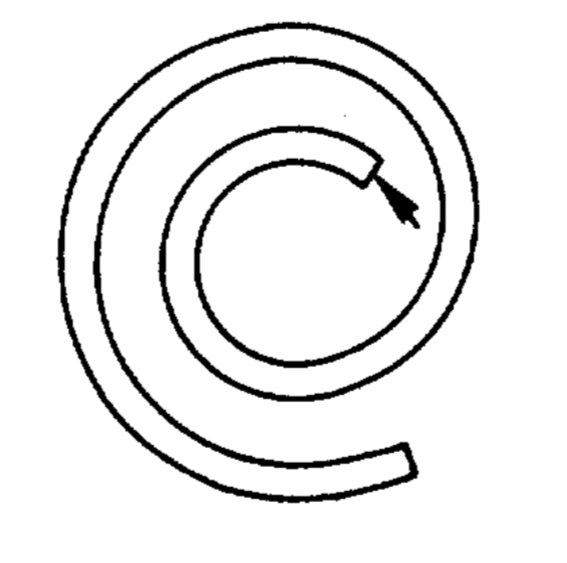
\includegraphics[scale=0.3]{img/mccloskey_1980_fig1b.png}
\end{center}
\section{Exercise}
The diagram shows a thin curved metal tube.
Imagine you are looking down the tube.
A metal ball is put into the end of the tube indicated by the arrow.
The ball is then shot out of the other end of the tube at high speed.
Please draw the past the ball will follow after it comes out of the tube \citep{mccloskey:1980_curvilinear}.
 
\section{Forms}
What is an Aristotelian form?
It ‘is not a subset of the properties that the organism [or thing] has, but rather a set of those that are 
proper to it, and towards which it strives or tends. Why does an acorn develop into an oak rather than 
a pig? Because of its special relation to the form that defines oak: it develops as it does because, 
while still an acorn, it lacks some of the properties that oaks have, and is somehow drawn towards 
instantiating that form more fully’ \citep[p.~10]{bennett:2003_learning}.
 
\section{Key Quote from \emph{Meditations}}
 
‘I have been in the habit of misusing the order of nature. For‘the proper purpose of [...] sensory perceptions [...] is simply to inform the mind of what is beneficial or harmful [...]; 
 and to this extent they are sufficiently clear and distinct. 
 But I misuse them by treating them as reliable touchstones for immediate judgements about the essential nature of the bodies located outside us; 
 yet this is an area where they provide only very obscure information.’ 
\citep[pp.~57-8]{descartes:1985_csm2}
 
\section{Impetus}
 
The person who sets the ball moving impresses in it a certain impetus,
[which acts] in the direction toward which the mover was moving the body,
either up or down, or laterally, or circularly’ (Buridan, 13xx; cited by McCloskey et al).
 
\section{Perceiving Impetus}
 
Sometimes when adult humans observe a moving object that disappears, they will misremember the location of its disappearance in way that reflects its momentum; this effect is called \emph{representational momentum} \citep{freyd:1984_representational,hubbard:2010_rm}.
 
The trajectories implied by representational momentum reveal that the effect reflects impetus mechanics rather than Newtonian principles \citep{freyd:1994_representational,kozhevnikov:2001_impetus,hubbard:2001_representational,hubbard:2013_launching}.
And these trajectories are independent of subjects' scientific knowledge
\citep{freyd:1994_representational,kozhevnikov:2001_impetus}.
Representational momentum therefore reflects judgement-independent expectations about objects’ movements which 
track momentum in accordance with a principle of impetus.%
\footnote{
Note that momentum is only one of several factors which may influence mistakes about the location at which a moving object disappears \citep[p.\ 842]{hubbard:2005_representational}.
%:
%\begin{quote}
%`The empirical evidence is clear that (1) displacement does not always correspond to predictions based on physical principles and (2) variables unrelated to physical principles (e.g., the presence of landmarks, target identity, or expectations regarding a change in target direction) can influence displacement.'
%
%...
%
%`information based on a naive understanding of physical principles or on subjective consequences of physical principles appears to be just one of many types of information that could potentially contribute to the displacement of any given target'
%\end{quote}
}
 
‘the representational momentum memory shift for a ball following a spiral path after exiting a tube is greater than the memory shift for a ball following the physically correct linear path. A curvilinear path, midway between the spiral and straight paths, produces shifts midway between those for the other two paths’
\citep[p.~975]{freyd:1994_representational}
 
Yet ‘our subjects had relatively accurate conscious knowledge of the trajectory of a ball exiting 
a spiral tube (63% to 83% chose the correct path; only 4% chose the spiral path).’
\citep[p.~975]{freyd:1994_representational}
 
‘subjects showed a memory shift for a path that the majority of subjects did not consciously consider correct’
\citep[p.~975]{freyd:1994_representational}
 
Aristotelian physics ‘is reasonably effective for organizing bodies of knowledge. From the 
perspective of modern physical and biological science, however, it is severely crippled by 
its close linkage with what Wilfrid Sellars calls ‘the manifest image’, i.e. what is available 
to us by means of our very limited sense organs. . . . The tie to entities known through 
perception prevents access to—much less the discoveries of—modern physics (and, consequently, 
chemistry and biology)’
(Turnbull 1988, p. 120 cited by \citealp{bennett:2003_learning}.)
 
\section{Books}
Core text: \citep{descartes:1985_csm2}.

Useful background (find one you like):
\begin{itemize}
\item Broughton, Janet 2002. Descartes' Method of Doubt. (Princeton University Press)
\item Hatfield, G. 2014. Descartes’ Meditations [The Routledge Guidebook to]. London: Routledge. 
\item Newman, Lex "Descartes' Epistemology", The Stanford Encyclopedia of Philosophy (Winter 2016 Edition), Edward N. Zalta (ed.).
\item Williams, B. 1978. Descartes: The Project of Pure Inquiry. Hassocks: Harvester Press. 
\item Wilson, Margaret. 1978. Descartes (Routledge).
\end{itemize}
\emph{Tip}: Hatfield is an invaluable reference. Any time you write about a 
passage from the Mediations, check what Hatfield writes about that passage.


    
    

% --------------
% ---- end paste
% --------------


% \vfill

% \

% \columnbreak

% \ 
% \vfill

\footnotesize
\bibliography{$HOME/endnote/phd_biblio}

\end{multicols*}

\end{document}
